{\fontsize{12pt}{22pt} \textbf{Overfitting}\par}

\vspace{5mm}

\newcommand{\quotes}[1]{``#1''}

\quotes{Overfitting occurs when our hypothesis fits the training data "too well"}. From Understanding Machine Learning - From Theory To Algorithms. \\

\begin{center}
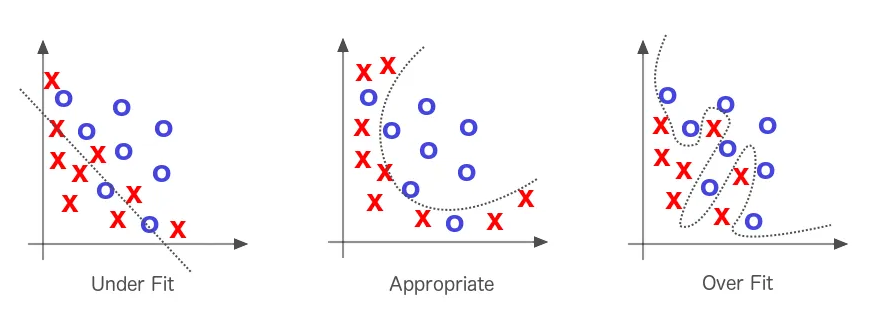
\includegraphics[scale=0.4]{overfitting.png}
\end{center}

Let $S$ be a training set and $\mathcal{D}$ a probability distribution.
An algorithm $A$ overfits if the difference between the \textit{true risk} of its output $\mathcal{L}_{\mathcal{D}}(A(S))$ and the \textit{empirical risk} of its output $\mathcal{L}_S(A(S))$ is large. \\

\textit{Note}: Recall from the \hyperref[sec:bias-complexity-trade-off]{bias-complexity trade-off} that overfitting is also when $\epsilon_{app}$ (error made by the best predictor) is low and thus $\epsilon_{est}$ (difference between the error of the best predictor and the error of the used predictor) is high. \\

\underline{Stability} \\

An algorithm is stable if a small change in input gives a small change in output. \\

Let $S^{(i)}$ be a training set where we replace the \textit{i-th} element by $z'$: $S^{(i)}=(z_1,...,z_{i-1}, z', z_{i+1}, ... , z_m)$. We measure an effect of a small change comparing the losses $\ell(A(S^{(i)}),z_i)$ and $\ell(A(S),z_i)$ ($z_i$ is the predicted value). 

We note that the algorithm trained on $S^{(i)}$ doesn't observe $z_i$ while the algorithm trained on $S$ does. Intuitively, we should have $\ell(A(S^{(i)}),z_i) - \ell(A(S),z_i) \geq 0$. \\

$A$ is stable on average if $\mathbb{E}_{(S,z') \sim \mathcal{D}^{m+1}, i \sim U(m)}[\ell(A(S^{(i)}),z_i) - \ell(A(S),z_i)]$ is small.

\vspace{5mm}